% vim: spelllang=en_gb

\documentclass[12pt,a4paper,draft]{scrartcl}
\usepackage{ifdraft}

% --------------------
% Set Language Options
% --------------------

\usepackage[nswissgerman,french,main=english]{babel}
\usepackage[autostyle,english=american,german=swiss]{csquotes}
\MakeOuterQuote{"}

\usepackage[shortcuts]{extdash}

% --------------
% Font & Symbols
% --------------

\usepackage[warnings-off={mathtools-colon,mathtools-overbracket}]{unicode-math}
\usepackage[oldstyle,proportional]{libertinus}

% ---------------
% Set Page Layout
% ---------------

% Get length of 65 characters
%\setlxvchars

\usepackage[driver=auto]{geometry}
% A5: 148mm × 210mm
% A4: 210mm × 297mm
\geometry{
  width=140mm,
  height=217mm,
  marginparsep=3mm,
  marginparwidth=30mm,
}
\ifdraft{\geometry{
  inner=10mm,
  marginparwidth=50mm
}}{}


% ---------------------
% Load Various Packages
% ---------------------

% Various Math Environments
\usepackage{mathtools}
\usepackage{amsthm,thmtools}
\usepackage{physics} % various shortcuts

% Bibliography
\usepackage{biblatex}
\addbibresource{bibliography.bib}

% For general figures
\usepackage[final]{graphicx}
\graphicspath{{/img}}
\usepackage{subcaption}
\usepackage{tikz}
\usetikzlibrary{babel,cd,shapes}
\tikzcdset{arrow style=math font}
\tikzset{cross/.style={cross out, draw, solid, thin, 
         minimum size=2*(#1-\pgflinewidth), 
         inner sep=0pt, outer sep=0pt},
         cross/.default={3}}

% For lists
\usepackage[shortlabels]{enumitem}

% For better Tables
\usepackage{tabularray}

% For more fine grained typesetting in final mode.
% Else set the tolerance for overfull warnings higher.
\ifdraft{\hfuzz=1.5pt}{\usepackage{microtype}}

% Links and stuff
\usepackage[final]{hyperref}
\usepackage[noabbrev]{cleveref}

% For Todonotes
\usepackage[obeyDraft]{luatodonotes}

% --------------------------------------------
% Define Theorem Environments & Math Operators
% --------------------------------------------

\declaretheorem[numberwithin=section]{theorem}
\declaretheorem[sibling=theorem]{lemma, proposition, corollary}
\declaretheorem[sibling=theorem,style=definition]{definition, example}
\declaretheorem[sibling=theorem,style=remark]{remark}

\DeclareMathOperator{\im}{im}
\DeclareMathOperator{\Aut}{Aut}
\DeclareMathOperator{\Diff}{Diff}
\DeclareMathOperator{\GL}{GL}
\DeclareMathOperator{\HF}{HF}
\DeclareMathOperator{\HM}{HM}
\DeclareMathOperator{\Hom}{Hom}
\DeclareMathOperator{\Ext}{Ext}
\DeclareMathOperator{\Tor}{Tor}

\begin{document}
\title{Exotic Tori from ATFs oder so}
\author{JoJoJo}

\maketitle

\section{Introduction}

\begin{definition}
  Let $k ∈ ℕ$ such that $0<k≤d$ and $a ∈ (0,∞)$. Through nodal slides we can arrange the ATF on $B_{dpq}$ such that the line $x₂=a$ intersects the branch cut line between the $(k-1)$-th and $k$-th degenerated fibre. $T_k(a)$ is defined to be the fibre over the intersection point of these two lines.
\end{definition}

\begin{theorem}
    \label{thm:bdpqexotic}
  Let $U ⊂ H¹(T_k(a),ℝ) ∖ \{\text{branch cut line}\}$.
  The restriction of the displacement energy germ to $U$ is given by
  \[ \eval{S_{T_k(a)}^e}_U (x,y) = a+\max\{x,x(1-kpq)-kp²y\}\todo{so oder so ähnlich…} \]
\end{theorem}


Let \(d,p,q ∈ ℕ\) such that \(d≥\) and \(p,q\) coprime with \(1≤q<p\) or \(q=0,p=1\), and \(0<a_1<…<a_d\) real integers.
Let \(P\) be the polynomial \(P(z) = \prod_{i=1}^d (z^p-a_i)\).
Define the manifold \(M_P\) by
\[M_P = \qty{(z_1,z_2,z_3) ∈ ℂ³ \mid z₁z₂ + P(z₃)=0 } \; .\]
We define the Hamiltonian system
\[\symbf{H}(z_1,z_2,z_3) = \qty(\abs{z_3}^2, \frac{1}{2}\qty(\abs{z_1}^2-\abs{z_2}^2))\]

Let \(ρ_p\) be the group of \(p\)-th roots of unity acting on \(M_P\) by
\[ρ \cdot (z₁,z₂,z₃) = \qty(ρz₁,ρ^{-1}z₂,ρ^q z₃), \quad ρ ∈ ρ_p \; .\]
This is a free  action, so we can define the quotient \(B_{dpq} = M_P/ρ_p\). The Hamiltonian system \(\symbf{H}\) is invariant under the action, so it descends to a Hamiltonian system on \(B_{dpq}\).
As in \cite[Chapter 6]{evans2021atfs}, we can remove a ray going through the critical values in the moment image, and use the flux map to obtain a moment map \(μ\) generating a Hamiltonian torus action everywhere except on the critical points, and having moment image \(Δ_{B_{dpq}}\) as in \cref{fig:Bdpq_moment_image}.\todo{Kann man besser formulieren.}

The position of the nodes can be varied along this ray by nodal slides.\todo{…which only affect some ε-neighboorhood.}

\begin{figure}
  \centering
  \begin{tikzpicture}[scale=.7]
    \fill[black!5] (0,4) rectangle (8,-2);

    \draw[thick,dotted,->] (2,1) node[cross] {} -- (4,2) node[cross] {} -- (8,4) node[anchor=west] {\((p,q)\)};
    \draw[thick] (0,4) -- (0,-2);
  \end{tikzpicture}
  \caption{Moment image of \(B_{dpq}\) under \(μ\)}
  \label{fig:Bdpq_moment_image}
\end{figure}


\section{Homology of \texorpdfstring{$B_{dpq}$}{Bdpq}}
\label{sec:homology}

In order to calculate the lower bound for the displacement energy of a Lagrangian fibre torus \(T(x,y) = μ^{-1}(\qty{(x,y)})\), we will need to calculate a basis for \(H_2\qty(B_{dpq},T(x,y))\).

\(B_{dpq}\) deformation retracts to the preimage of the branch cut line segment \(l\) shown in red in \cref{fig:branch_cut_retraction}, by first vertically shrinking the space onto the ray in direction \((p,q)\), and then compressing the part of the ray that is to the right of all the critical points.
\todo{Das ist etwas dumm formuliert, lohnt es sich das besser zu formulieren?}

The preimage \(μ^{-1}(l)\) can be understood as follows: If there were no critical points on the line, this would be a solid torus \(T = S¹×D²\).
We pick \((1,0),(0,1) ∈ H₁(∂T)\) to be the classes generated by \(S¹×\text{pt},\text{pt}×∂D²\) respectively.
For each critical fibre \(k ∈ \qty{1,…,d}\) we collapse a loop along the homology class \((-q,p)\), as in \cref{fig:collapse_cycles}.
Up to homotopy this is the same as attaching a disk \(D_k\) along \((-q,p)\).
Again up to homotopy we can also require that the \(d\) discs \(D_1,…,D_d\) are attached along \(∂T\).
Let us call this space $S$.

\begin{figure}
  \centering
  \begin{subfigure}{0.45\textwidth}
    \centering
      \begin{tikzpicture}[scale=.7]
      \begin{scope}[fill=black!5]
        \fill[clip] (0,4) rectangle (8,-2);

        \draw[black!30, very thick] (0,0) -- (8,4);
        \draw[red,line width=.125cm,draw opacity=.5, line cap=round] (0,0) -- (4,2) node[anchor=north] {\(l\)};
        \draw[thick,dotted] (2,1) node[cross] {} -- (4,2) node[cross] {} -- (8,4);
      \end{scope}
      \draw[thick] (0,4) -- (0,-2);
    \end{tikzpicture}
    \caption{Retraction to branch cut line}
    \label{fig:branch_cut_retraction}
  \end{subfigure}%
  \begin{subfigure}{0.55\textwidth}
    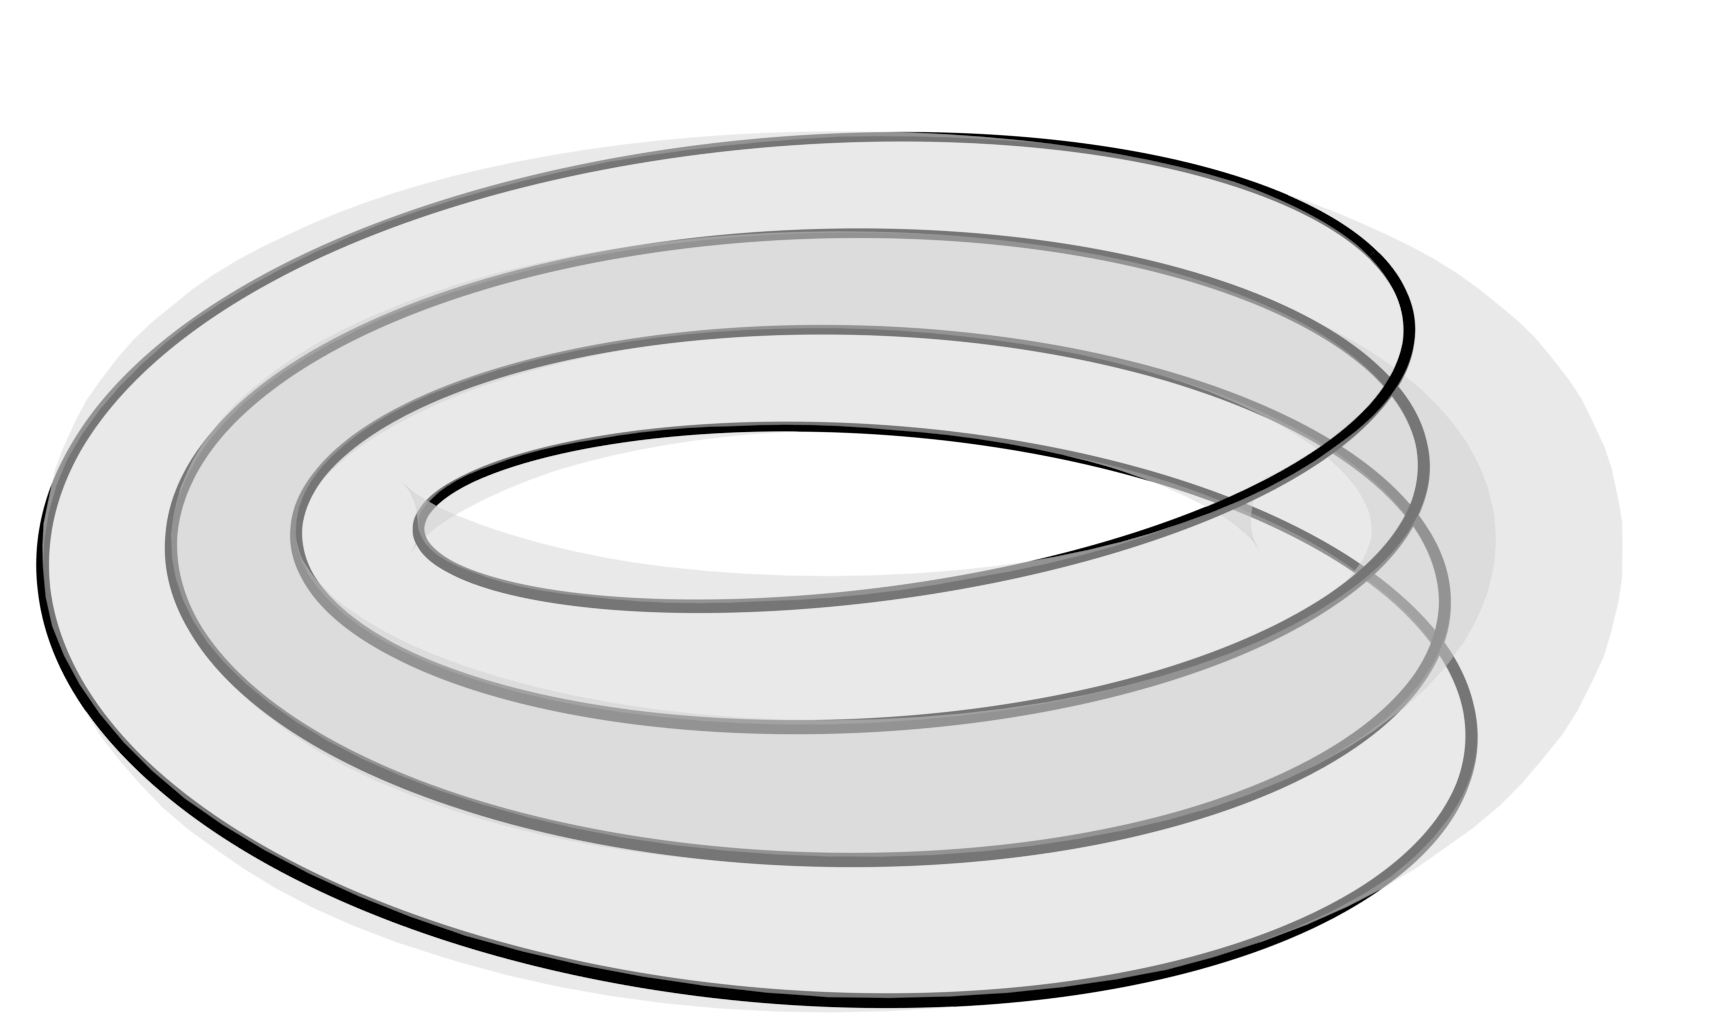
\includegraphics[width=\textwidth]{img/homology_collapse.png}
    \caption{The cycles marked in black (here \(p=2, q=1\)) are collapsed to a point.}
    \label{fig:collapse_cycles}
  \end{subfigure}
  \caption{Calculation of the homology of \(B_{dpq}\)}
\end{figure}

Let us look at the long exact sequence of homology for the pair \(\qty(B_{dpq},T(x,y))\). This pair is homotopy equivalent to \((S,∂T)\).

\[
\begin{tikzcd}
  H_2(∂T) \ar[r,"0"] &
  H_2(S) \ar[r,hook]\ar[d,"≅"] &
  H_2(S,∂T) \ar[r]\ar[d,"≅"] &
  H_1(∂T) \ar[r]\ar[d,"≅"] &
  H_1(S) \ar[d,"≅"]
  \\
  &
  ℤ^{d-1} &
  ℤ^{d+1} &
  ℤ² &
  ℤ_p
\end{tikzcd}
\]

The first horizontal map is zero since \(∂T\) retracts to a circle in \(S\).
The homology \(H_2(S)\) can be seen as follows: By contracting the solid torus \(T\) in \(S\) to a circle, we see that \(S\) is homotopic to a circle with \(d\) discs glued to its boundary by a degree \(p\) map.
So \(H_2(S)\) is generated by spheres \(\qty{S_2,…,S_d}\), \(S_k = D_{k-1}-D_{k}\).
\(H_2(S,∂T)\) is generated by the discs \(D_0 = \text{pt}×D²,D₁,…,D_d\). In \(B_{dpq}\), these discs can be seen, where the disc intersecting the toric boundary collapses the \((0,1)\) cycle in the toric fibre \(T(x,y)\) and the discs intersecting the critical points collapse the \((-q,p)\) cycle (see \cref{fig:homology_generating_discs}).
The elements $S_2,\ldots,S_d \in H_2(B_{dpq})$ can be realized by embedded Lagragian spheres fibering over the segments between the nodes in the ATF -- these are so-called \emph{visible Lagrangians}, see \cite[section 7.4]{evans2021atfs}.
The boundary map $∂ \colon H_2(S,∂T) → H_1(∂T)$ is given by $\partial D_0 = (0,1),\, \partial D_i = (-q,p)$, meaning that the last horizontal map \(H_1(∂T) → H_1(S)\) maps $(0,1)$ to the generator of $ℤ_p$.


\begin{figure}
  \centering
  \begin{tikzpicture}
    \fill[black!5] (0,4) rectangle (7,-1);

    \coordinate (xy) at (2.7,3.5);
    \node[anchor=south] at (xy) {\(T(x,y)\)};
    \fill (xy) circle[radius=.05];
    \draw (xy)
           .. controls +(0,0) and +(-.5,1) .. node[anchor=east, near end] {\(D₁\)} (2,1)
      (xy) .. controls +(0,0) and +(-.5,1) .. node[anchor=west, near end] {\(D₂\)} (4,2)
      (xy) .. controls +(0,0) and +(-.5,1) .. node[anchor=west, near end] {\(D₃\)} (6,3)
      (xy) .. controls +(0,0) and +(1,0) .. node[anchor=south, near end] {\(D₀\)} (0,2.5);

    \draw[ultra thick, blue, draw opacity=.3] (2,1) -- node[anchor=north] {\(S₂\)} (4,2);
    \draw[ultra thick, purple, draw opacity=.3] (4,2) -- node[anchor=north] {\(S₃\)} (6,3);

    \draw[thick,dotted] (2,1) node[cross] {} -- (4,2) node[cross] {} -- (6,3) node[cross] {} -- (7,3.5);

    \draw[thick] (0,4) -- (0,-1);
  \end{tikzpicture}

  \caption{The disks \(D₀, …, D_d\) generating the homology \(H₂\qty(B_{dpq}, T(x,y))\)}
  \label{fig:homology_generating_discs}
\end{figure}

\section{Lower Bound on Displacement Energy: Minimal J-holomorphic Curves}

Let \(T(x,y)\) a fibre torus, where \((x,y)\) is not over the branch cut line. In \cite{chekanov1998} the following is proven:

\begin{theorem}
  \label{thm:chekanov}
  Let \((X,ω,J)\) be a \todo{tame/geometrically bounded} symplectic manifold with \(ω\)-tame almost complex structure \(J\). Let \(L ⊂ X\) be a compact Lagrangian submanifold. Then the displacement energy satisfies
  \[e(L) ≥ \min\qty{σ_D(X,L,J),σ_S(X,J)}\]
\end{theorem}


Fibres $T(λ p,λ q)$ for $λ > 0$ are monotone whenever they are not on a node. We compute displacement energy of the non-monotone fibres.\todo{das müsste man auch noch zeigen oder verrefferenzen, ist aber irgendwie irrelevant…}
Note that $T(x_0,y_0)$ yields a well-defined torus up to Hamiltonian isotopy, i.e.\ it is independent of the nodal slides, see \todo{referenz, kein guter platz hierfür}.

We want to use \cref{thm:chekanov} to find a lower bound, so first we need to choose a suitable almost complex structure on \(B_{dpq}\)

\subsection{Almost complex structure for \texorpdfstring{\(B_{dpq}\)}{Bdpq}}


\begin{proposition}
\label{prop:bdpq}
Let $T(x_0,y_0)$ be a non-monotone ATF-fibre of $B_{dpq}$.
Then it has displacement energy
\[e(B_{dpq}, T(x_0,y_0)) ≥ x_0 .\]
\end{proposition}

\begin{proof}
    We use \cref{thm:chekanov} together with \cref{lem:bdpqdisk}. 
\end{proof}

\todo{Add proof of \cref{thm:bdpqexotic}.}


\section{Buffer Zone Lemma}

Let \((n,a)\) be two coprime integers, \(ρ_n\) the group of \(n\)-th roots of unity. Let \(ρ_n\) act on \(ℂ^2\) by \(ρ(z₁,z₂) = ( ρ z_1,ρ^a z_2)\).
Let \(A(n,a) = ℂ^2/ρ_n\) be the quotient space.
This space is an orbifold, with one orbifold point at \([(0,0)]\).
The space \(S³/ρₙ\) is the lens space \(L(n,a)\), so \(A(n,a)\) is the cone over \(L(n,a)\).

We define the Hamiltonian system on \(A(n,a)\) by 
\begin{equation}
  \label{eqn:hamsysAna}
  \symbf{G}(z_1,z_2) = \frac{1}{2}\qty(\abs{z_2}², \frac{1}{n}\qty(\abs{z₁}²+a\abs{z₂}²)) \;.
\end{equation}

With this Hamiltonian system the moment polytope is a wedge with edges pointing along vectors \((1,0), (n,a)\), as seen in \cref{fig:Ana_moment_image}.
\(A(n,a)\) has a almost complex structure \(J\) descending from the canonical complex structure on \(ℂ²\).

We have the commutative diagram
\begin{equation}
  \label{eqn:Ana_commdiag}
  \begin{tikzcd}
    ℂ² \ar[r,"π"] \ar[d,"\symbf{H}"] & A(n,a) \ar[d, "\symbf{G}"] \\
    Δ_{ℂ²} \ar[r,"L_{A(n,a)}"] & Δ_{A(n,a)}
  \end{tikzcd}
\end{equation}
where the left vertical map \(\symbf{H}\) is given by \((z₁,z₂) ↦ \frac{1}{2}\qty(\abs{z_1}²,\abs{z_2}²)\), and the bottom map is a linear transformation given by the matrix
\[ L_{A(n,a)} = \mqty(0 & 1\\\frac{1}{n} & \frac{a}{n})\;.\]

\begin{figure}
  \centering
  \begin{tikzpicture}[scale=1.5]
    \draw[thick,fill=black!5,->] (0,2) -- (0,0) -- (3,2) node[anchor=south] {\((n,a)\)};
  \end{tikzpicture}
  \caption{Moment image of \(A(n,a)\) with given by Hamiltonian system \(G\)}
  \label{fig:Ana_moment_image}
\end{figure}

Let \(B(a) ∈ ℂ^n\) be the open ball in \(ℂ^n\) of radius \(\sqrt{\frac{a}{π}}\).
In \cite[appendix~A]{chekanovschlenk2015} the following lemma is proven:
\begin{lemma}
  \label{lem:hyperannulus}
  Let \(a_+ > a_- ≥ 0\).
  Let \(u \colon Σ → B(a_+)∖ \overline{B(a_-)}\) be a J-holomorphic curve such that the closure of \(u(Σ)\) in \(ℂ^n\)intersects \(∂B(a_-)\).
  Then \(∫_u ω ≥ a_+ - a_-\).
\end{lemma}

We give the slight generalization:

\begin{lemma}
  \label{lem:hyperannulus2}
  Let \(a_+ > a_- > 0\), and
  \[X = \symbf{G}^{-1}\qty(\qty{c₁(0,1)+c₂(n,a) \mid a_- < c₁ + c₂ < a_+}) ⊂ A(n,a) \;,\]
  equipped with the almost complex structure of \(A(n,a)\).

  Let \(u \colon Σ → X\) be a J-holomorphic curve whose closure intersects
  \[\symbf{G}^{-1}\qty(\qty{c₁(0,1)+c₂(n,a) \mid a_- = c₁ + c₂}) \; .\]

  Then \(∫_u ω ≥ a_+ - a_-\).
\end{lemma}

\begin{remark}
  \label{rem:hyperannulus3}
  Suppose we have a moment polytope \(Δ\) of a (almost) toric symplectic manifold or orbifold \(\symbf{H} \colon M → Δ\) with two non-parallel edges given by the two primitive vectors $u₁,u₂$, as in \cref{fig:cutting_out_a_hyperannulens}.
  Suppose without loss of generality that the edges intersect in the origin.
  Then the subset
  \[X = \symbf{H}^{-1}\qty(\qty{c₁u₁+c₂u₂ \mid a_- < c₁ + c₂ < a_+})\]
  with \(a_±\) such that \(a_± u₁, a_± u₂ ∈ Δ\), can be transformed by a \(T ∈ \GL(ℤ²)\), such that \(Tu₁=(0,1), Tu₂=(n,a)\), for some coprime integers \(n,a\).

  With this transformation we can view \(X\) as a subset of \(A(n,a)\). Equipping \(M\) with an extension of the almost complex structure coming from \(A(n,a)\), we get that J-curves in \(M\) intersecting
  \[\symbf{H}^{-1}\qty(\qty{c₁u₁+c₂u₂ \mid a_- = c₁ + c₂})\]
  must have at least area \(a_+ - a_-\).
\end{remark}

\begin{figure}
  \centering
  \missingfigure{Hyperannulens inside a moment polytope.}
  \caption{Hyperannulens \todo{\textbf{NOOOOOOOOOOOO!}} inside a moment polytope.}
  \label{fig:cutting_out_a_hyperannulens}
\end{figure}
\begin{proof}
  Since the action of \(ρ_n\) is free in \((ℂ^*)²\), the projection map \(π \colon (ℂ^*)² → A(n,a) ∖ \{[(0,0)]\}\) is an n-fold covering map.

  The using the commutative diagram \ref{eqn:Ana_commdiag}, we can compute the preimage
  \[
    π^{-1}(X) = (\symbf{H} ∘ L_{A(n,a)})^{-1}(\symbf{G}(X)) = B(na_+) ∖ B(na_-)\;.
  \]

  A J-curve \(u\colon Σ → A(n,a)\) lifts to a J-curve \(\tilde{u}\), i.e. a curve making the diagram
  \[
    \begin{tikzcd}
      Σ' \ar[r,"\tilde{u}"] \ar[d,"\tilde{π}"] & ℂ² \ar[d,"π"] \\
      Σ \ar[r,"u"] & A(n,a)
    \end{tikzcd}
  \]
  commute, where \(\tilde{π} \colon Σ' → Σ\) is some n-fold covering of \(Σ\).

  Using \cref{lem:hyperannulus}, we get that the symplectic area of \(\tilde{u}\) is at least \(n(a_+ - a_-)\), and since \(\tilde{u}\) is an n-fold covering of \(u\), \(u\) has at least symplectic area \(a_+-a_-\), as desired.

\end{proof}


\section{Upper bound on displacement energy: Probes}

\iffalse
%incomplete proof of Chekanov-Schlenk lemma
\begin{proof}
  Let \(r ∈ (a_-,a_+)\) such that the intersection \(u(Σ) ∩ ∂B_r\) is transversal.
  Then this intersection is an immersed 1-dimensional manifold, so it is a collection of immersed circles.
  Let \(γ\) be a parametrization of one of these circles.
  We choose a local holomorphic reparametrization of \(u\) as follows: 
  \begin{align*}
    \tilde{u} : S¹xI &→ ℂ^n \\
    u(t,0) &= γ(t)
  \end{align*} \todo{ja, was jetzt?}
  
  Then
  \begin{align*}
    F'(r) &= ∫_{u(Σ) ∩ ∂B_r} u^* ω \\
          &≥ ∫_{S¹} ω(\pdv{u∘s}{t},\pdv{u∘s}{r}) \dd t \\
          &= ∫_{S¹} ω(\pdv{u}{t}+\pdv{s}{t}\pdv{u}{s},\pdv{s}{r}\pdv{u}{s}) \dd t \\
          &= ∫_{S¹} \pdv{s}{r} ω(\pdv{u}{t},i \pdv{u}{t}) \dd t \\
          &= ∫_{S¹} \pdv{s}{r} \abs{\dot{γ}(t)}^2 \dd t \\
          &≥ l^2(γ) ∫_{S¹} \pdv{r}{s} \dd t
  \end{align*}

  Also
  \begin{align*}
    l^2(γ) &≥ ∫_{S¹} γ^* α_n = ∫_{S¹}⟨\dot{γ},ξ⟩ \dd t
  \end{align*}
\end{proof}
\fi


\printbibliography

\end{document}
